\vspace{-10pt}
\section{SIC Values and Correctness}

First, we evaluate the correlation between the \sic values of the output tuples and the correctness of
the computed results across a representative range of \emph{aggregate} and \emph{top-k} classes of
queries (see Table~\ref{table:queries}). 
The experiments use the synthetic workload as well as real load measurements collected on PlanetLab
(see Table~\ref{table:inputs}).
% Furthermore, we also include the calculation of the covariance
% metric between two time-series data of real numbers which is widely used in statistics and scientific processing to measure the correlation between two variable.
% \mnote{What are these time-series and where are they used? Probably there should be a citation.}
% 
% When using the SIC metric to provide feedback on processing quality to users,
% it is important that performance of the result of the query output is 
% \emph{strictly increasing} to the SIC values: \ie as the SIC values increase,
% the query result output is getting \emph{closer} to the perfect result 
% without shedding or it does not change. 
% \mnote{This text is from the paper. I agree on the ``stictly increasing'' argument.}
%
%\subsection*{Experimental Setup}

For this set of experiments the local testbed is used (see Table~\ref{table:machines}). A single \sys
processing node is overloaded by instantiating an increasing number of queries of one class. As we increase the number of queries, the node is forced to discard
more input tuples. The node uses a load-shedder that discards tuples randomly from each query.
The experiment is repeated for every query class and for each of the five different sets of source data. 
\vspace{-10pt}
\subsection*{Correlation Metrics}

We compare the results of a query with degraded processing (\ie with result SIC values of less
than~1) against the result of a query with perfect processing. Each query, degraded and perfect, runs
for 5~minutes and the error in the results is measured every second as a function of the achieved SIC
value. For each query class, the experiment is repeated for all the different input data sets.

%For the \textnormal{AVG}, \textnormal{COUNT} and \textnormal{MAX} aggregate 
For the \textnormal{AVG} and \textnormal{COUNT} aggregate 
queries, we use the \emph{mean absolute error} (MAE) to quantify the relative distance of the
\emph{degraded} from the \emph{perfect} result value across all
measurements for the duration of the experiment:
\vspace{-10pt}
\begin{align}
\text{MAE} = \frac{1}{n} \mathlarger{‎‎\sum}{\left\lvert {\displaystyle \frac{\displaystyle
\mathit{degraded} -
\displaystyle
\mathit{perfect}}{\displaystyle \mathit{perfect}}}} \right\rvert
\end{align}

For the \textnormal{TOP-5} query, we calculate the error using the
Kendall distance metric~\cite{kendall} that counts the differences (\ie permutations and
elements in only one list) of pairs of distinct elements between the two
lists. 
The Kendall's distance $\tau$ is defined as:
\begin{align}
\tau = \frac{C_p-D_p}{\frac{1}{2} n (n-1)}
\end{align}
where $C_p$ is the number of concordant pairs, $D_p$ is the number of discordant pairs and $n$ is the
total number of pairs. This value is normalised to lie within the [0,1] interval.

In the case of the \textnormal{COV} query, we compare the standard deviation of the real covariances
with the one under overload. The real covariance comes from perfect processing, and its value is matched
with the covariance obtained for degraded processing. Hence, we can evaluate the correlation between the
\sic values and the quality of the \textnormal{COV} query results.
% The duration of each experiment is 5~minutes each and the \textnormal{COV} query outputs a new
% \emph{sample} covariance every 1~sec. 
  
%--------------------------------------------------------------------------------------------------------
\subsection*{Experimental Results}
The following graphs show the results from the experiments running queries belonging to the
\emph{aggregate} and \emph{complex} classes. A graph is shown for each query type (\textnormal{AVG},
\textnormal{COUNT}, \textnormal{TOP-5} and \textnormal{COV}). Each graph contains the
measurements from the different runs of the experiment, one for each input data~set.

\paragraph{Aggregate queries.}
For the \textnormal{AVG} queries (see Figure~\ref{fig:agg-avg}), the graph shows a small error even
under heavy overload. This is due to the particular nature of the average operation. Since the
load-shedder discards tuples at random, the distribution of the data is not significantly affected. 
However, we observe that, as the amount of \mbox{load-shedding} diminishes and the SIC values increase,
the degraded values are closer to the perfect ones.

The \textnormal{COUNT} query (see Figure~\ref{fig:agg-count}) shows a different behaviour. The error
grows linearly with the amount of discarded data. This is an extreme case, in which the occurrence of
\mbox{load-shedding} has always a direct effect on the final results. Each tuple that is discarded, in fact,
reduces the total output value (\ie the final count) and thus increases the error.
\vspace{15pt}
% In the case of the \textnormal{MAX} query (see Figure~\ref{fig:agg-max}), we note that the result has a
% small error for the synthetic distributions. However, the error increases and shows a linear correlation in the
% case of the mixed and the PlanetLab distributions. The reasons for this difference in behaviour could be
% due to the different nature of the data sets. In the uniform, exponential and gaussian data sets, the
% data is arranged according to a regular distribution, thus a random reduction of the input data does not 
% modify the difference in absolute terms. For the PlanetLab and Mixed data sets instead, the input values
% are more scattered and have a lower regularity. \todo
% ---- AVG FIGURE -----
\begin{figure}[h!]
\centering
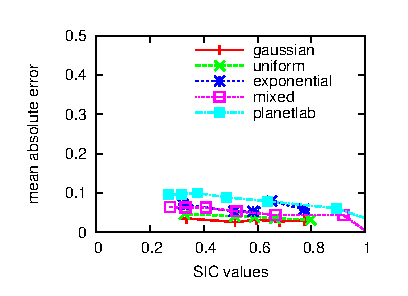
\includegraphics[width=0.55\textwidth]{img/tesi/avg1}
\caption{Correlation of SIC values with the query output quality for \emph{average} queries.}
\label{fig:agg-avg}
\end{figure} 
\clearpage

% ---- COUNT FIGURE -----
\begin{figure}
\centering
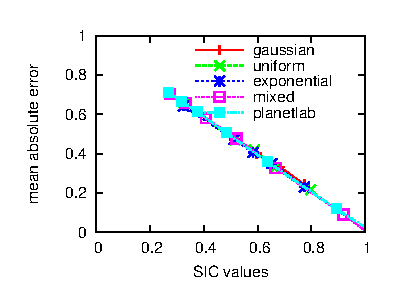
\includegraphics[width=0.55\textwidth]{img/tesi/count1}
\caption{Correlation of SIC values with the query output quality for \emph{count} queries.}
\label{fig:agg-count}
\end{figure}
% % ---- MAX FIGURE -----
% \begin{figure}
% \centering
% \label{fig:max}
% 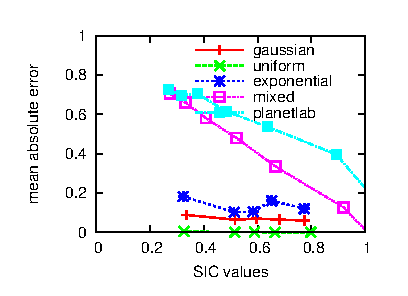
\includegraphics[width=0.6\textwidth]{img/tesi/max1}
% \caption{Correlation of SIC values with the query output performance for \emph{Max} queries.}
% \label{fig:agg-max}
% \end{figure}
%--------------------------------------------------------------------------------------------------------
\paragraph{Complex queries.}
For the \textnormal{TOP-5} query (see Figure~\ref{fig:top5}), the error expressed as the Kendal distance
decreases almost linearly with the amount of \mbox{load-shedding} performed, showing a good correlation
between the \sic metric and the correctness of results for this type of query. 
%The abnormal data point in the exponential distribution is most probably an outlier, due to some
%undetected problem with the experimental setup.

For the \textnormal{COV} query (see Figure~\ref{fig:cov}), the standard deviation of results shows a
decreasing trend as the amount of \mbox{load-shedding} diminishes and the \sic value increases. This means that
when the amount of overload is reduced, the spread in the value of the results is also reduced.
All input distributions, real and synthetic, show a low error despite the large amount of
\mbox{load-shedding}. 
% Only the exponential distribution suffers from a larger error, even with limited overload.
% This behaviour is due to the nature of the data distribution. \todo

Even for this other set of queries, the experimental results show a good correlation between the achieved
\sic values and the correctness of the results. The severity of the overload condition is, in general,
directly proportional to the error observed in the output results. This means that, although the \sic
metric is designed as a generic quality metric, it provides a good indication of the quality of the
computed results.
\begin{figure}[h!]
\centering 
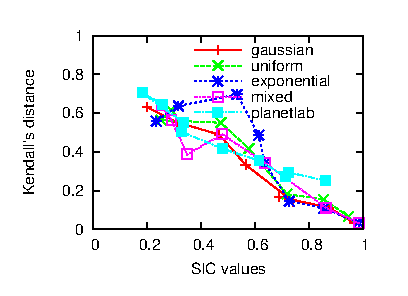
\includegraphics[width=0.55\textwidth]{img/tesi/topK-distance}
\caption{Correlation of the SIC values with the query output quality for \emph{top-5} queries.}
\label{fig:top5}
\end{figure}
\clearpage
% ---- COVARIANCE FIGURE -----
\begin{figure}[h!]
\centering
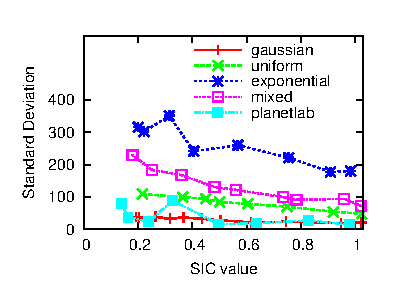
\includegraphics[width=0.55\textwidth]{img/tesi/cov}
\caption{Correlation of the SIC values with the query output quality for \emph{covariance} queries.}
\label{fig:cov}
\end{figure}% The results show that there in most cases there is a strictly increasing 
% correlation between the result SIC values and the distance/error to the perfect result: 
% the more the SIC values increase, the smaller the error. The degree of correlation 
% depends on the type of query and the source data
% distribution. When tuples are discarded randomly, tuples with values across the
% range of the initial distributions are chosen at random. The distribution of
% the values of admitted tuples are correlated with the original distribution.